%\documentclass[notes]{beamer}       % print frame + notes
%\documentclass[notes=only]{beamer}   % only notes
\documentclass{beamer}              % only frames
\usepackage[default]{sourcesanspro}
\usepackage[ngerman]{babel}
\usepackage[utf8]{inputenc}
\usepackage{graphicx}
\usepackage{ccicons}

\usetheme{default}
\usebeamercolor{wolverine}
\useoutertheme{smoothbars}

\beamertemplatenavigationsymbolsempty{}

\setbeamertemplate{footline}[text line]{%
  \parbox{\linewidth}{\vspace*{-8pt}Datensouveräne Web-Anwendungen mit der Solid-Technologie\hfill\insertpagenumber}}
        
\setbeamercolor{title}{fg=black}
\usepackage[inkscapearea=page]{svg}
\usepackage[edges]{forest}
\usepackage{longtable,booktabs} %Tabellen mit zeilenumbruch
\usepackage{subcaption}
\definecolor{LightGray}{rgb}{0.97,0.97,0.97}
\definecolor{codegreen}{rgb}{0,0.6,0}
\definecolor{codegray}{rgb}{0.5,0.5,0.5}
\definecolor{codepurple}{rgb}{0.58,0,0.82}

\usepackage{listings}
\lstdefinestyle{rdf}{
    commentstyle=\color{codegreen},
    keywordstyle=\color{magenta},
    numberstyle=\tiny\color{codegray},
    stringstyle=\color{codepurple},
    basicstyle=\ttfamily\tiny,
    breakatwhitespace=false,         
    breaklines=true,                 
    captionpos=b,                    
    keepspaces=true,                                  
    showspaces=false,                
    showstringspaces=false,
    showtabs=false,                  
    tabsize=2
}

\lstset{style=rdf}


\title{Datensouveräne Web-Anwendungen mit der Solid-Technologie}

\author{Anna Denzel, Alexander Reiprich, Istvan J. Mocsy}
\subtitle{Modul “Software Engineering” (Prof. Dr. Andreas Both, Wintersemester 2023/2024) an der HTWK Leipzig}
\date{\today}
\begin{document}

{
	\usebackgroundtemplate{%
			
\includegraphics[width=\paperwidth]{images/balkengreen.png}
		}
\begin{frame}[plain]

\includegraphics[height=3ex]{images/HTWK_Zusatz_de_H_Black_K.eps}
 \titlepage{}
 \cczero
\end{frame}
}

\makeatletter
\patchcmd{\endbeamer@frameslide}{\ifx\beamer@frametitle\@empty}{\iffalse}{}{\errmessage{failed to patch}}
\makeatother

\makeatletter
\setbeamertemplate{frametitle}{%
	\ifbeamercolorempty[bg]{frametitle}{}{\nointerlineskip}%
	\@tempdima=\textwidth%
	\advance\@tempdima by\beamer@leftmargin%
	\advance\@tempdima by\beamer@rightmargin%
	\begin{beamercolorbox}[sep=0.0cm,left,wd=\the\@tempdima]{frametitle}
		\raisebox{-0.15cm}{
\includegraphics[width=0.0212\paperwidth]{images/headergreen.png}}
		\begin{minipage}{.81\paperwidth}
			\usebeamerfont{frametitle}%
			\vbox{}\vskip-1ex%
			\if@tempswa\else\csname beamer@fteleft\endcsname\fi%
			\strut\insertframetitle\par%
			{%
				\ifx\insertframesubtitle\@empty%
				\else%
				{\usebeamerfont{framesubtitle}\usebeamercolor[fg]{framesubtitle}\strut\insertframesubtitle\par}%
				\fi
			}%
		\end{minipage}%
		\enspace\quad\qquad\raisebox{-0.15cm}{
\includegraphics[width=0.0212\paperwidth]{images/headergreen.png}}
		\if@tempswa\else\vskip-.3cm\fi% set inside beamercolorbox... evil here...
	\end{beamercolorbox}%
}
\makeatother 

\begin{frame}	
	\frametitle{Gliederung}
	\tableofcontents
\end{frame}

\section{Geschichte}
\begin{frame}{Geschichte}
\begin{figure}[htbp]
    \centering
    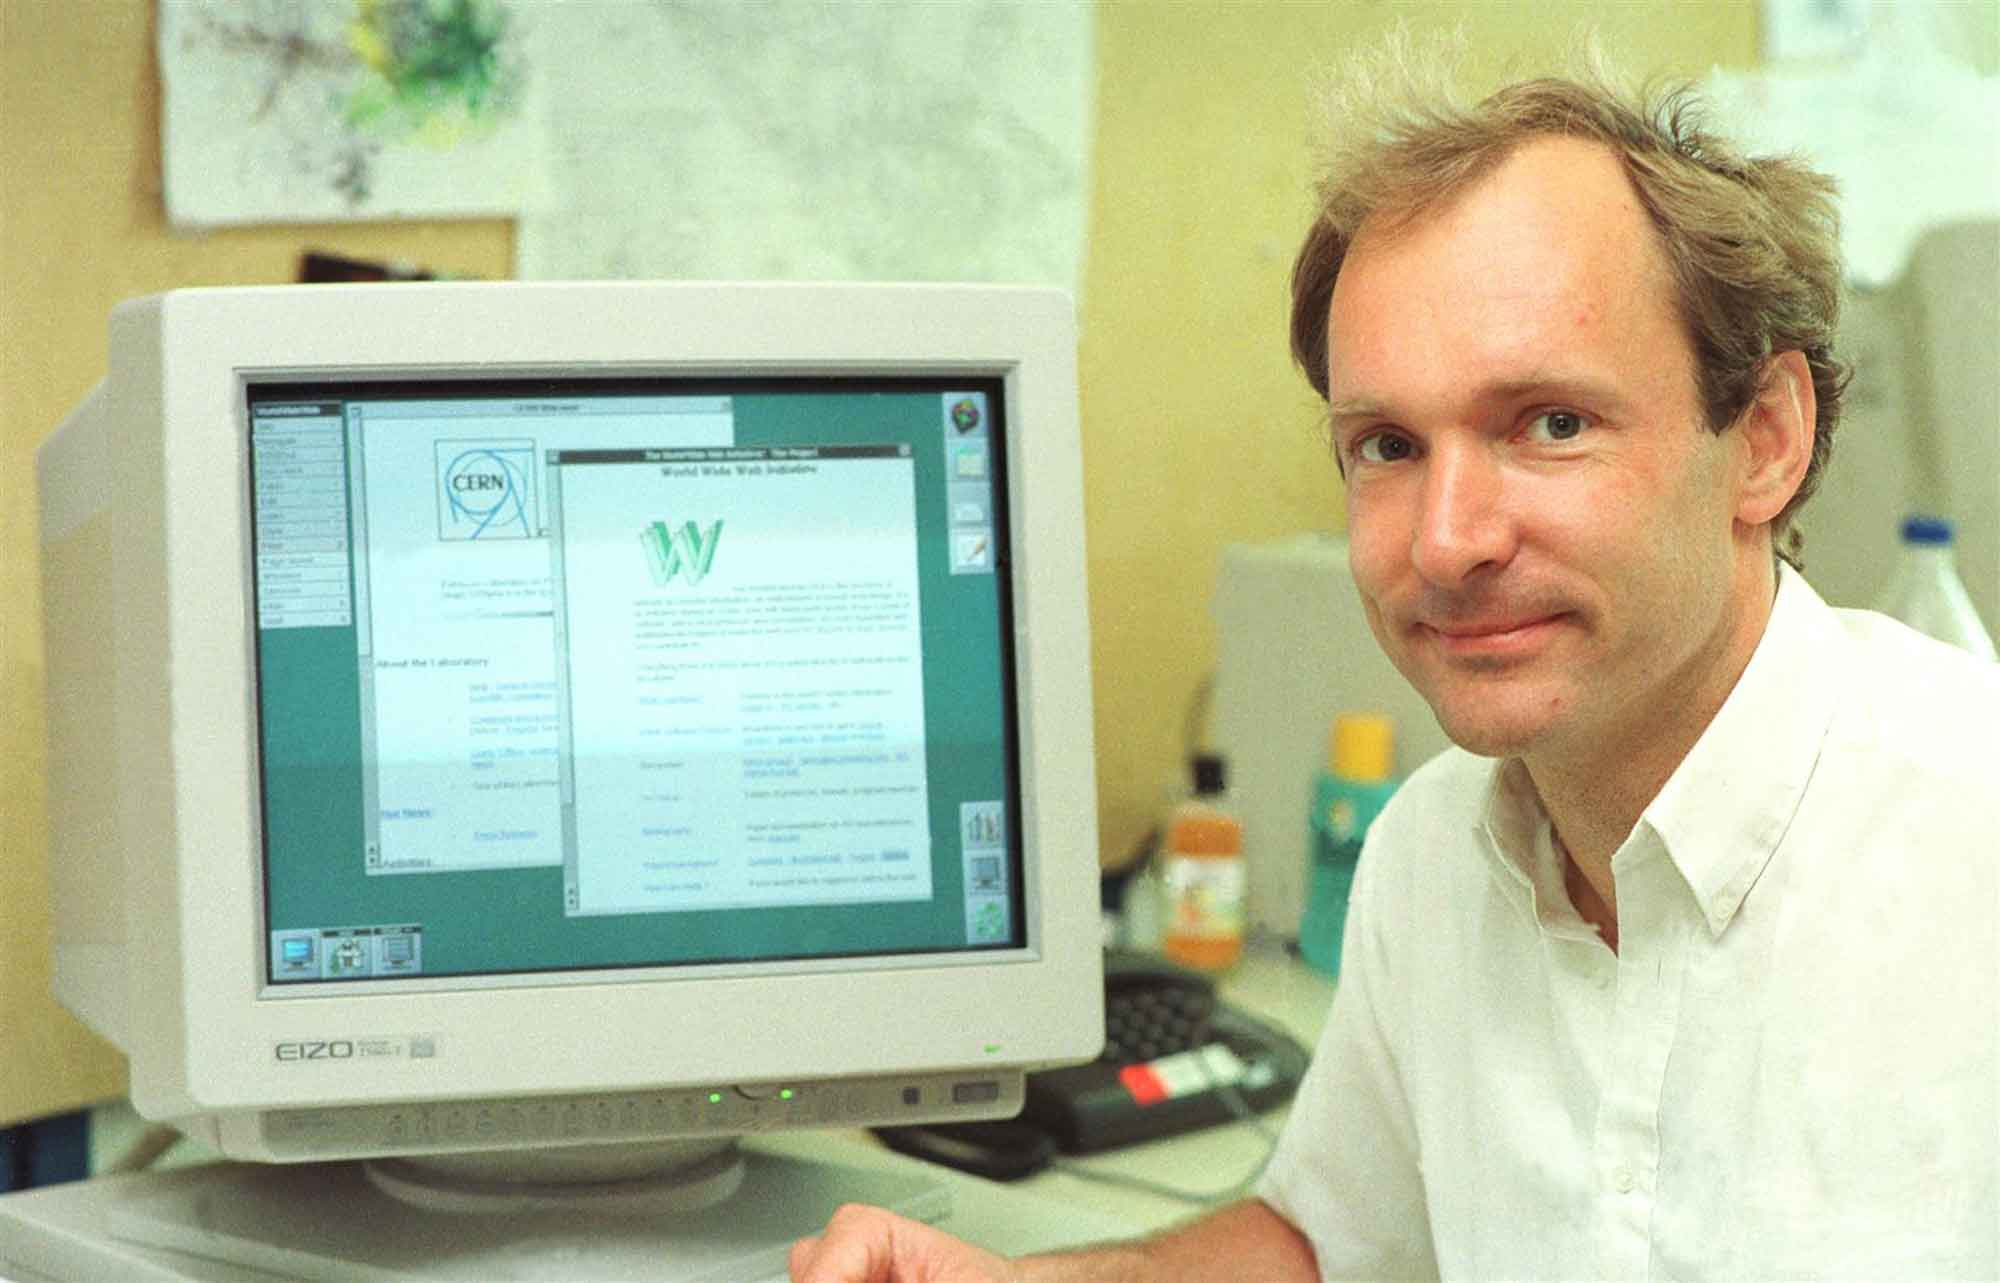
\includegraphics[width=0.70\paperwidth]{images/berners-lee.jpg}
    \caption{Tim Berners-Lee, 1994 in CERN}
    \url{http://cds.cern.ch/record/39437\#31}
\end{figure}
\end{frame}

\section{Zentralisiertes Konzept}
\begin{frame}{Zentralisiertes Konzept}
\begin{figure}[htbp]
\centering
\includesvg[width=0.45\paperwidth]{images/centralized_concept.svg}
 \caption{Aufbau des zentralisierten Konzepts: Nutzer gibt Daten an verschiedene Anwendungen}
 \end{figure}
\end{frame}
\begin{frame}{Limitierungen und Probleme des zentralisierten Konzept}
\begin{itemize}
    \item Kontrollverlust über die Daten (Überwachungskapitalismus) \cite{zuboff2018ueberwachungskapitalismus}
    \item Veraltete, unvollständige Datensätze oder duplizierte Datensätze 
    \item Kontinuierlicher Managementaufwand
    \item Hohe Einstiegshürde für neue Unternehmen
    \item Verlust der Innovation, da keine Konkurrenzfähigkeit ohne Datensilos
\end{itemize}
\end{frame}

\section{Solid - Social Linked Data}
\begin{frame}{Der Beginn von Solid}
\begin{itemize}
    \item Semantic Web und Linked Data Konzepte \cite{bernerslee1998semanticwebroadmap}
    \item "Three challenges for the web, according to its inventor"  \cite{webfoundation2017}
    \item Berners-Lee ruft Solid (Social Linked Data) ins Leben
\end{itemize}
\end{frame}

\subsection{Grundlagen Solid}
\begin{frame}{Grundlagen von Solid\cite{MarcoNeumann.2021}}
\begin{figure}[htbp]
  \centering
  \includesvg[width=0.70\paperwidth]{images/concepts.svg}
  \caption{Zentralisiertes Anwendungen besitzen Daten des Users, Dezentralisierte Anwendungen fragen bei User an, ob Sie Datenzugriff erhalten können}
\end{figure}
\end{frame}

\begin{frame}{Datenverteilung\cite{MarcoNeumann.2021}}
\begin{figure}[htbp]
  \includesvg[width=0.80\paperwidth,inkscapelatex=false]{images/datasilos.svg}
  \caption{Zentralisierte Webanwendungen besitzen verschiedene Versionen der selben Information, während dezentralisierte Webanwendungen auf die Pods zugreifen}
\end{figure}
\end{frame}

\begin{frame}{Kommunikation der Anwendungen und Daten\cite{MarcoNeumann.2021}}
\begin{figure}[htbp]
  \includesvg[width=0.80\paperwidth,inkscapelatex=false]{images/backends.svg}
  \caption{Zentralisierte Anwendungen besitzen ein angepasstes Backend, während dezentralisierte Anwendungen höhere Interoperabilität besitzen}
\end{figure}
\end{frame}

\begin{frame}{Das Solid-Ökosystem}
%Todo: Grafik die zeigt wie man mit Solid ein Netz an Komponenten aufbauen (Anwendung, Authentification, Data Pod)
\begin{figure}[htbp]
  \includesvg[width=0.80\paperwidth,inkscapelatex=false]{images/ecosystem.svg}
  \caption{Interaktionen der einzelnen Komponenten im Solid-Ökosystem\cite{soliddeblackboxed}}
\end{figure}

\end{frame}

\begin{frame}{Das Solid-Ökosystem: Begriffe}
\begin{itemize}
    \item Podprovider: Service welcher Pod bereitstellt und i.d.R. Identität überprüft \cite{sambra2016solid}
    \item WebID: Ressource, welche einen Pod im Solid-Ökosystem identifiziert
    \item Access Control List (ACL): Regelt die Zugriffsberechtigungen für die Ressourcen eines Pods
    \item Solid App: Anwendung, welche nach den Vorgaben des Solid-Protokolls aufgebaut ist
\end{itemize}
\end{frame}

\subsection{Semantic Web}
\begin{frame}{Semantic Web}
\begin{itemize}
    \item W3Cs Vision eines "Web of Linked Data" \cite{bernerslee1998semanticwebroadmap}
    \item Technologiestack um Linked Data zu beschreiben und zu verarbeiten
    \item Zuweisung von Uniform Resource Identifier (URI) für Ressourcen \cite{blumauer2006semantic}
    \item Beschreibung von Datenzusammenhang über Ontologien \cite{staab2009handbook}
    \item Speicherung von Daten als Knowledge Graph (KG) \cite{blumauer2006semantic}
\end{itemize}
\end{frame}

\subsection{Resource Description Framework (RDF)}
\begin{frame}{Resource Description Framework (RDF)}
\begin{itemize}
    \item URI: Eindeutiger Bezeichner einer Ressource, oft ähnlich einer URL \cite{blumauer2006semantic}
    \item Ressource: \texttt{\dq Sache\dq} über die Aussage getroffen werden soll, eindeutig bezeichnet \cite{blumauer2006semantic}
    \item Literal: Zeichenkette, die Daten enthält
    \item Ontologie/Vokabular: Datei, welche Zusammenhänge zwischen Ressourcen beschreibt \cite{staab2009handbook}
    \item Knowledge Graph: Datei, welche die Ressourcen als Tripel zu eben diesen Graphen zusammensetzt \cite{staab2009handbook}
\end{itemize}
\end{frame}

\begin{frame}{Resource Description Framework (RDF)}
\begin{figure}[htbp]
  \centering
  \includesvg[width=0.8\paperwidth]{images/rdftripelvocab.svg}
  \caption{Zusammenhang zwischen Ressource, Tripel, Ontologie und KG}
\end{figure}
\end{frame}

\subsubsection{Linked Data}
\begin{frame}{Linked Data}
\begin{figure}[htbp]
  \centering
  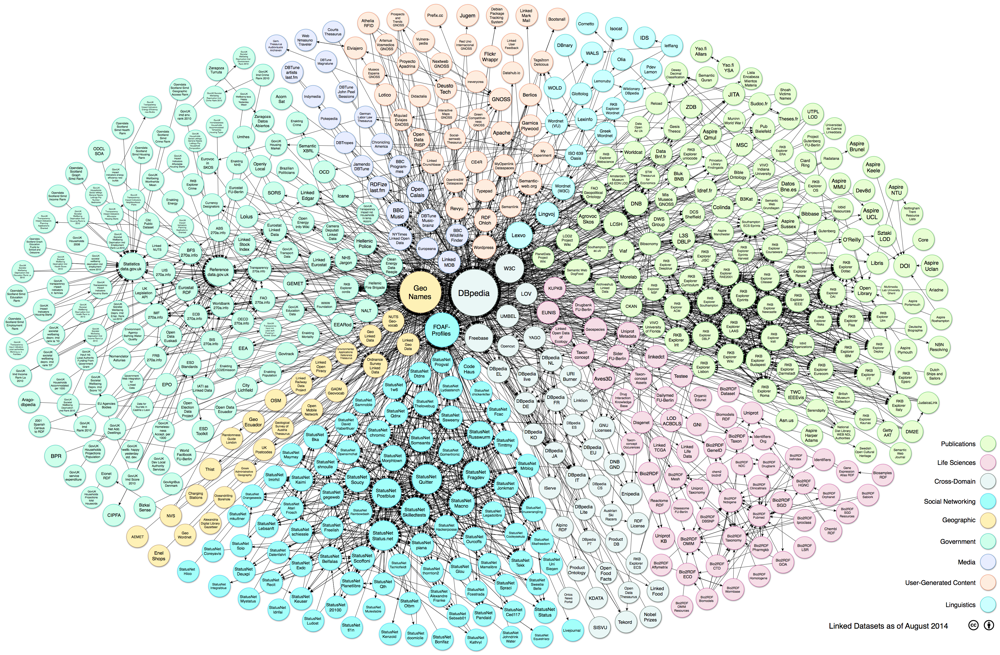
\includegraphics[width=0.55\paperwidth]{images/linked-data.png}
  \caption{Linked Open Data Cloud, circa 2016}
\end{figure}
\url{https://medium.com/openlink-software-blog/what-is-dbpedia-and-why-is-it-important-d306b5324f90}
\end{frame}

\subsection{Solid Anwendungsbeispiel}
\begin{frame}{Anwendungsbeispiel}
\begin{figure}[htbp]
  \centering
  \includesvg[width=0.8\paperwidth]{images/solidflixneu.svg}
\end{figure}
\end{frame}

\subsubsection{Daten in Solid}
\begin{frame}[fragile]{Ressource in Solid}
\begin{minipage}{\linewidth}
\begin{lstlisting}[captionpos=b, caption=Ressource des Films Zurück in die Zukunft II welche in einem Pod abgelegt wurde., label=lst:ressourcebttf2,frame=single]
@prefix example: <https://pods.solidcommunity.au/example#> .
@prefix dct:     <http://purl.org/dc/terms/> .
@prefix xsd:     <http://www.w3.org/2001/XMLSchema#> .
@prefix schema:  <https://schema.org/#> .

example:movies/back-to-the-future-part-ii#it
    dct:created         "2024-01-24T09:51:05.553Z"^^xsd:dateTime;
    dct:modified        "2024-01-24T09:51:05.553Z"^^xsd:dateTime;
    a                   schema:WatchAction;
    
    schema:name         "Back to the Future Part II";
    schema:description  "Marty and Doc are at it again in this wacky sequel to the 1985 blockbuster as the time-traveling duo...";
    schema:image        "http://image.tmdb.org/t/p/original/hQq8xZe5uLjFzSBt4LanNP7SQjl.jpg?api_key=e70f4a66202d9b5df3586802586bc7d2";
    schema:datePublished "1989-11-22T00:00:00.000Z"^^xsd:dateTime;
    schema:sameAs       "https://www.themoviedb.org/movie/165", "https://www.imdb.com/title/tt0096874".
\end{lstlisting}
\end{minipage}
\end{frame}

\subsection{Vorteile}
\begin{frame}{Vorteile}
\begin{itemize}
    \item Großes Skalierungspotential \cite{8633673}
    \item Trennung Daten und Webanwendungen mit Kommunikation über Schnittstellen (hohe Interoperabilität) \cite{8633673}
    \item Datenverwaltung durch Nutzer:innen (Data Privacy) \cite{yeung2023decentralization} 
    \item Keine veralteten Datensätze \cite{MarcoNeumann.2021}
    \item Datensouveränität
    \item Feingranulare Autorisierung und sichere Authentifizierung \cite{acp.2022}
\end{itemize}
\end{frame}

\begin{frame}{Potential für Unternehmen}
\begin{itemize}
    \item Niedrigere Entwicklungskosten durch Auslagern vieler Funktionalitäten 
    \item Einfache Modularisierung und Integration von Funktionalitäten
    \item Kein Daten- und Identitätsmanagement mehr notwendig
    \item Kein legale Begrenzungen für Datenspeicherung \cite{MarcoNeumann.2021}
    \item Zugriff auf aktuelle Datensätze der Nutzer:innen \cite{MarcoNeumann.2021}
    \item Raum für Innovationen \cite{MarcoNeumann.2021}
\end{itemize}
\end{frame}


\subsection{Nachteile}
\begin{frame}{Pitfalls und Gefahren}
\begin{itemize}
    \item Falsche Umsetzung des Konzepts (Missbrauch von Daten) \cite{MarcoNeumann.2021}
    \item Erhöhte technische Komplexität \cite{MarcoNeumann.2021}
    \item Andere Implementierung der Kommunikation notwendig \cite{MarcoNeumann.2021}
    \item Große Umstellung für Entwickler:innen und Nutzer:innen \cite{MarcoNeumann.2021}
    \item Performance-Probleme (Kommunikation mit mehreren Modulen/Pods notwendig -> sehr viele Netzwerkzugriffe) \cite{MarcoNeumann.2021}
    \item Referenz auf Daten nicht beständig und keine garantierte Zugriffsberechtigung
\end{itemize}
\end{frame}

\section{Ausblick}
\begin{frame}{Ausblick}
Drei Einsatzmöglichkeiten von Solid:
\begin{itemize}
    \item Gesicherte Verifizierung mit Blockchain ~\cite{ramachandran2020towards}
    \item Solid Data Spaces ~\cite{meckler2023web}
    \item ConSolid für Linked Building Data ~\cite{8633673}~\cite{werbrouck2022consolid}
\end{itemize}
\end{frame}

\section{Zusammenfassung}
\begin{frame}{Zusammenfassung}
Solid...
\begin{itemize}
    \item ...ist eine Alternative zum aktuellen zentralisierten Konzept der Datenverwaltung.
    \item ...nutzt das Resource Description Framework (RDF) um Daten und Ressourcen zu speichern.
    \item ...bietet Nutzer:innen und Unternehmen mehr Kontrolle über die eigenen Daten durch die Nutzung von Personal Online Datastores (Pods).
    \item ...erlaubt hohe Interoperabilität durch die freie Kombinierbarkeit von Pods, Providern und Anwendungen.
\end{itemize}
\end{frame}

\section{Diskussion}
\begin{frame}{Diskussion}
1. Was wäre ein guter Umgang mit Ressourcen, welche von einem Podnutzer nicht mehr zur Verfügung gestellt werden, zu welcher aber Referenzen bestehen?


2. Was wären mögliche Anwendungsfälle, die von dem dezentralisierten Ökosystem profitieren würden?
\end{frame}

\section{Quellen}
\begin{frame}[allowframebreaks]
        \frametitle{Quellen}
        \bibliographystyle{abbrv}
        \bibliography{bibliography}
\end{frame}

\section{Lizenz}
\begin{frame}{}
   \centering Diese Belegarbeit ist unter der CC0 1.0 Universal lizensiert. \url{https://creativecommons.org/publicdomain/zero/1.0/}
\end{frame}
\end{document}

% {Copypasta für Bilder, weil man die Syntax eh jedes mal googled wie ein verdammter Ersti}:

% \begin{frame}
% 	\begin{columns}
% 	\column{.5\linewidth}
%     \begin{figure}
%         \centering
%         \includegraphics[width=0.35\paperwidth]{intent.png}
%         \caption{Beispiel Intent}
%         \label{fig:intt}
%     \end{figure}
%     \column{.5\linewidth}
%         \begin{figure}
%         \centering
%         \includegraphics[width=0.35\paperwidth]{rasastory.png}
%         \caption{Beispiel Story}
%         \label{fig:stry}
%     \end{figure}
%     \end{columns}
% \end{frame}


% {Copypasta für Codeblocks, weil man die Syntax eh jedes mal googled wie ein verdammter Ersti}:

% \begin{frame}[fragile]
% \frametitle{Beispiel Taxifahrt-Daten}
% \rule{\textwidth}{1pt}
% \tiny
% \begin{minted}{python}
% def extract_taxi_data() -> [[str, pd.DataFrame]]:
%     dfs_taxi_data = []

%     for taxi_type in config.TAXI_TYPES:
%         df_taxi_type: pd.DataFrame = pd.DataFrame()

%         for year in config.TAXI_YEARS:
%             filename = str(year) + "_" + taxi_type + ".csv"
%             df_year = pd.read_csv(path.join(config.DATA_PATH, filename))

%             df_taxi_type = pd.concat([df_taxi_type, df_year], ignore_index=True)
%             logger.success("{filename} extracted.", filename=filename)

%         dfs_taxi_data.append([taxi_type, df_taxi_type])

%     logger.success("Taxi data extracted.")
%     return dfs_taxi_data
% \end{minted}
% \rule{\textwidth}{1pt}
% \end{frame}